\chapter{Pol~III \abbr{chip}-sequencing quantifies \abbr{trna} gene
expression}
\label{sec:chip}

\section{Quantifying expression of \abbr{trna} genes}

We quantified \trna gene expression via \pol3 \chipseq. The reason for using
this, on the first glance indirect, measure is caused by the fact that \trna
genes are unfortunately not identifiable by their sequence alone: performing a
multiple sequence alignment of \trna genes in \mmu reveals that several \trna
genes share the exact same sequence.

\textfloat{trna-alignment}{spill}
    {\footnotesize\begingroup
\let\m\mismatch
\begin{tabular}{@{}ll@{}}
    \toprule
    chr5.trna1044 &  \seq{GTCTCTGTGGCGCAATCGGTtAGCGCGTTCGGCTGTTAACCGAAAG...........GtTGGTGGTTCGAGCCCACCCAGGGACG}\\
    chr3.trna750 &   \seq{GTCTCTGTGGCGCAATCGGTtAGCGCGTTCGGCTGTTAACCGAAAG...........GtTGGTGGTTCGAGCCCACCCAGGGACG}\\
    chr3.trna298 &   \seq{GTCTCTGTGGCGCAATCGGTtAGCGCGTTCGGCTGTTAACCGAAAG...........GtTGGTGGTTCGAGCCCACCCAGGGACG}\\
    chr3.trna294 &   \seq{GTCTCTGTGGCGCAATCGGTtAGCGCGTTCGGCTGTTAACCGAAAG...........GtTGGTGGTTCGAGCCCACCCAGGGACG}\\
    chr3.trna289 &   \seq{GTCTCTGTGGCGCAATCGGTtAGCGCGTTCGGCTGTTAACCGAAAG...........GtTGGTGGTTCGAGCCCACCCAGGGACG}\\
    chr2.trna1947 &  \seq{GTCTCTGTGGCGCAATCGGTtAGCGCGTTCGGCTGTTAACCGAAAG...........GtTGGTGGTTCGAGCCCACCCAGGGACG}\\
    chr1.trna1014 &  \seq{GTCTCTGTGGCGCAATCGGTtAGCGCGTTCGGCTGTTAACCGAAAG...........GtTGGTGGTTCGAGCCCACCCAGGGACG}\\
    chr11.trna1446 & \seq{GTCTCTGTGGCGCAATCGGTtAGCGCGTTCGGCTGTTAACCGAAAG...........GtTGGTGGTTCGAGCCCACCCAGGGACG}\\
    chr10.trna390 &  \seq{GTCTCTGTGGCGCAATCGGTtAGCGCGTTCGGCTGTTAACCGAAAG...........GtTGGTGGTTCGAGCCCACCCAGGGACG}\\
    chr3.trna757 &   \seq{GTCTC\m CGTGGCGCAAT\m CGGT\m cAGCGCGTTCGGCTGTTAACCGAAAG...........GtTGGTGGTTCGAGCCCACCC\m GGGGACG}\\
    chr3.trna283 &   \seq{GTCTCTGTGGCGCAATTGGTtAGCGCGTTCGGCTGTTAACCGAAAG...........GtTGGTGGTTC\m AAGCCCACCCAGGGACG}\\
    \bottomrule
\end{tabular}
\endgroup

    \todo{Fix alignment of table}}
    {Alignment of Asn \trna genes.}
    {Parts of a multiple sequence alignment of \trna genes in \mmu generated
    with COVE\@. Shown are the \trna genes coding for Asn. Bases which differ
    from the consensus sequence are highlighted in red.}

In order to identify individual \trna genes and quantify their expression, we
therefore cannot resort to conventional \rnaseq: the \rna reads covering only
the transcribed gene region are indistinguishable. Common strategies for
counting ambiguously mapping reads, as used in \name{ERANGE} by
\citet{Mortazavi:2008}, still require at least \emph{some} unambiguous
information, to distinguish different genes which share reads.
\todo{Biological background of pol3 ChIP}

We solve this problem by extending the \trna gene body into the flanking
regions, which are not under purifying selection, and therefore not conserved.
As \pol3 \chipseq fragments cover the flanking regions as well as the actual
gene body (\cref{fig:trna-pol3-binding-profile}), we can use reads uniquely
mapping to the flanking regions in order to extrapolate coverage of the gene
bodies for ambiguous reads (\cref{fig:trna-pol3-map-ambiguous-reads}).

\textfig{trna-pol3-binding-profile}{spill}{\textwidth}
    {\trna \pol3 \chip binding profile.}
    {The shaded, bell-shaped area shows an idealised binding profile of \chipseq
    data spanning the \trna gene with the A and B box highlighted, as well as
    its flanking regions upstream and downstream of the gene body. This overlap
    plays a role in identifying the individual gene.}

When mapping the reads, we therefore do not discard all ambiguously mapping
reads. However, we still discard reads which are likely \pcr duplicates, i.e.\
map to more locations than there are possible \trna genes sharing a common
sequence (we more or less arbitrarily used the threshold of \num{20} non-unique
mapping locations). We thus end up with reads which have not been assigned to a
given \trna gene (\cref{fig:trna-pol3-map-a}). In order to assign
these reads to \trna genes, we reassign reads after mapping, using the number of
uniquely mapping reads in \trna genes’ flanking regions to determine the most
likely origin (\cref{fig:trna-pol3-map-b}) \citep{Kutter:2011}.

Let \(i\) be the \(i\)th \trna gene locus, and \(c_i\) be the count of
uniquely mapped reads in its flanking region (we used \SI{\pm100}{bp}). A
multi-mapping read \(r\), which maps to a set \(T\) of candidate \trna[s], can
be allocated to a target \trna gene \(i\) randomly with probability

\begin{equation}
    p_i = \begin{cases}
        c_i\left(\sum_{x \in T}c_x\right)^{-1} &
            \text{if \(\sum_{x \in T}c_x \neq 0\),} \\
        \vert T \rvert^{-1} & \text{otherwise.}
    \end{cases}
\end{equation}

\textfloat{trna-pol3-map-ambiguous-reads}{spill}{%
    \centering
    \begingroup
        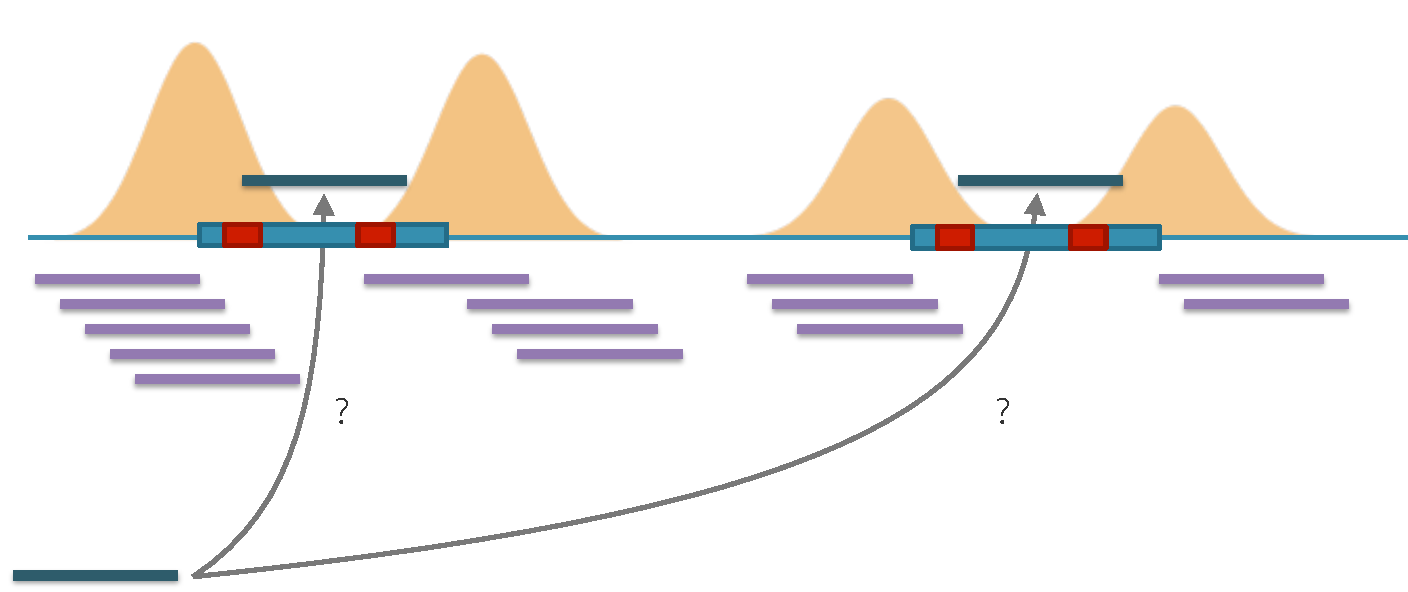
\includegraphics[width=\textwidth]{trna-pol3-map-ambiguous-reads-1}
        \subcaption{\label{fig:trna-pol3-map-a}Two potential match candidate
            \trna genes for a read.}
    \endgroup
    \begingroup
        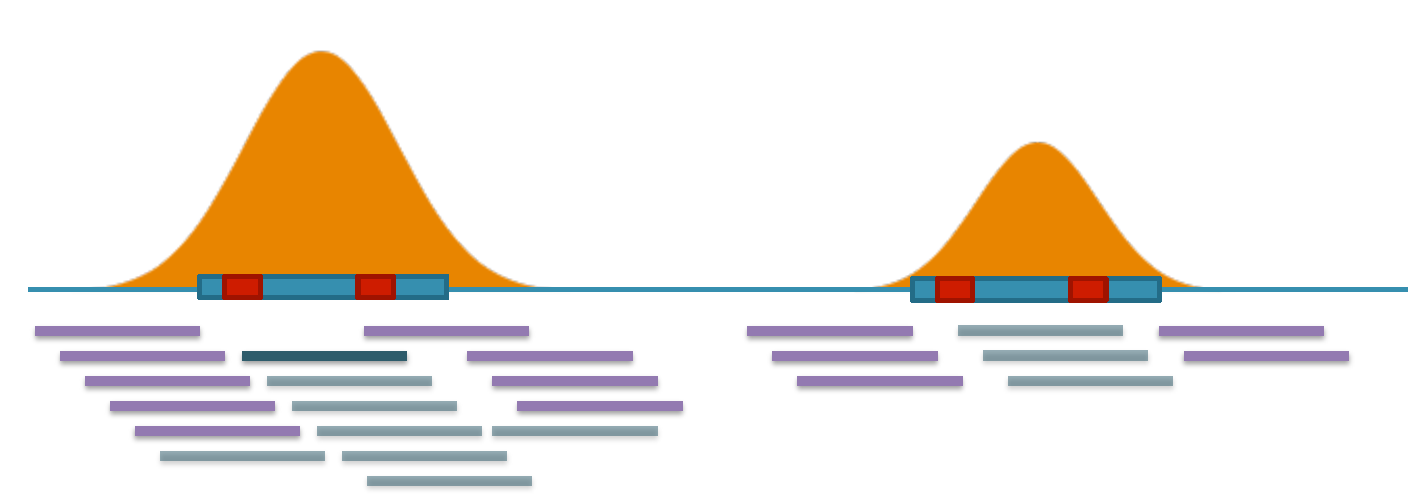
\includegraphics[width=\textwidth]{trna-pol3-map-ambiguous-reads-2}
        \subcaption{\label{fig:trna-pol3-map-b}Using the count data from the
            flanking regions to extrapolate most likely mapping positions for
            ambiguous reads.}
    \endgroup}
    {Mapping ambiguous \chip reads.}
    {\chip reads originating from \trna genes can often not be mapped
    unambiguously to any given \trna. Instead, information form the gene’s
    flanking regions is used to determine the more likely provenance.}

Quantification of \trna genes was performed by first mapping the \pol3 \chipseq
data (non-strand-specific \SI{36}{bp} single-end reads sequenced by
\name{Illumina} \name{Genome Analyzer~IIx} or \name{HiSeq~2000}) using
\name{BWA} version 0.5.9-r16 \citep{Li:2009a} using default parameters. Next,
non-uniquely mapping reads were reallocated probabilistically according to the
description given above, using the \trna gene annotation from the \name{Genomic
\trna Database}, described in \citet{Chan:2009}. For each \trna gene (excluding
mitochondrial \trna genes), reads were summed on each \trna gene locus and in
the \SI{\pm100}{bp} flanking regions.

\trna genes that were unexpressed in all our experimental conditions were
excluded from the analysis, in order to reduce the effect of multiple testing
\citep{Bourgon:2010}, and to exclude potential pseudogenes in the annotation. To
be called expressed, a \trna gene had to be present in all replicates of at
least one condition with a count of at least \num{10}, after size-factor
normalisation. The threshold \num{10} was chosen so that small variations in
either direction would have a minimal impact on the thresholding.

%\section{Normalisation of \trna gene expression}
%
%Raw \trna gene expression counts show strong differences between sequencing
%libraries. For \mrna count data, it is customary to use \name{DESeq}’s
%\dfn{library size normalisation} \citep{Anders:2010}. However, as shown in
%\cref{fig:trna-libraries-example}, library size normalised data still follows
%distinct distributions, which we deem biologically implausible, and probably due
%to technical bias.
%
%As a consequence, we opted to \dfn{quantile normalise} the count data\todo{find
%reference for quantile normalisation}.
%
%\textfloat{trna-libraries-example}{body}
%    {\centering\Huge Placeholder}{Placeholder}{Placeholder}
